In this project I used Python version 2.7.

Python is a widely-used, general-purpose programming language as shown in
figure \ref{python-popularity}. Python focuses on human readability, simplicity
and power to the programmer.\cite{website:python-zen,website:python-faq-creation-reason} That fact is most likely best expressed by the fact that Python uses indentation to divide its blocks. A
language like C uses the curly braces for that and uses the indentation only for
clarity of reading. Python, however, forces the programmer to make the program
more readable and standardised. Semantically Python is very flexible. It
supports functional, object-oriented and procedural programming styles.

%\usepackage{graphics} is needed for \includegraphics
\begin{figure}[htp]
\begin{center}
  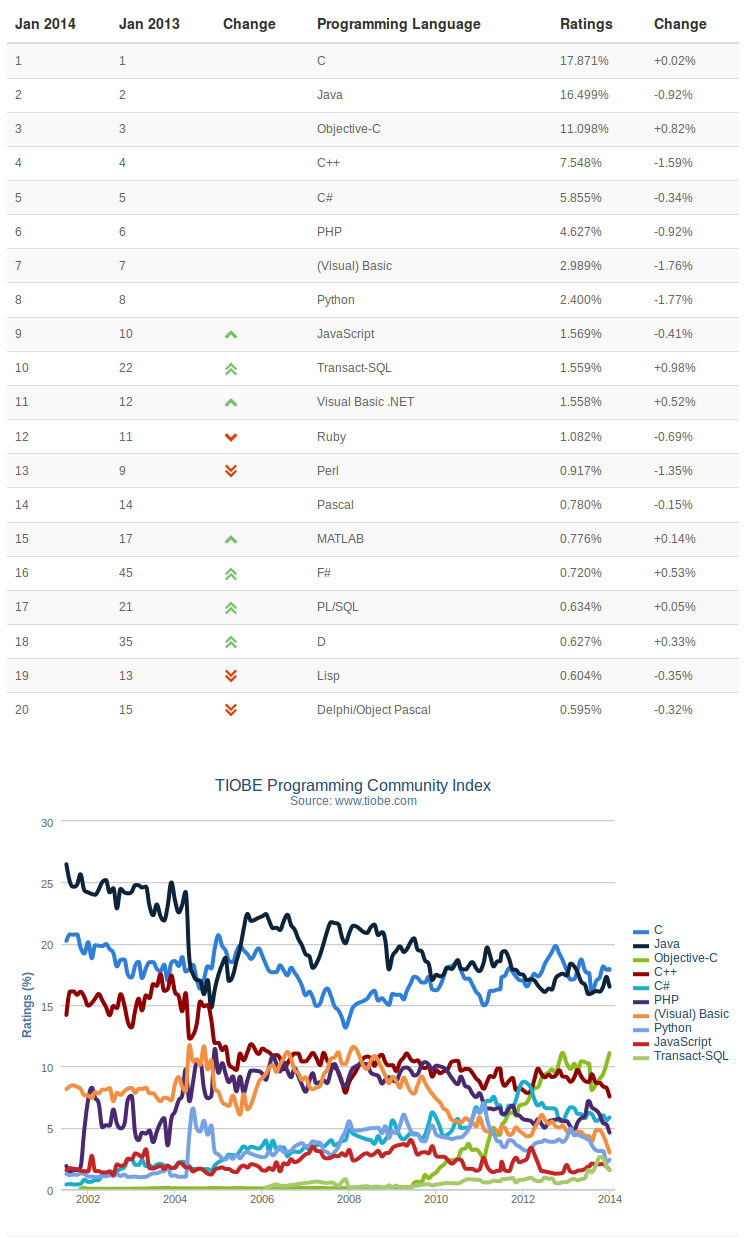
\includegraphics[height=564pt]{tiobe}
  \caption[Python popularity]{Popularity of python compared to other
  languages\cite{website:tiobe-index}}
  \label{python-popularity}
\end{center}
\end{figure}

To minimise clutter in the language, Python uses dynamic typing, also called
duck typing. Duck typing doesn't check if an object implements some certain
interface, but simply tries to call or use the method or attribute. The
principle is ``If it looks like a duck and quacks like a duck, it must be a
duck''.\cite[duck-typing]{website:python-glossary} This makes it possible to not use
interfaces and generics in the code.

Python has two running modes: the interactive mode and the script mode. The
interactive mode is a read-eval-print loop. It reads the user supplied
expression and parses it into a data structure, evaluates it and prints the
result. An expression can't be multiline and must return only one value.
Evaluating a value will return that value and evaluating a variable returns the
contents of the variable. The script running mode is similar to the interactive
mode, but instead of the user, the expressions are taken from a file and when
the end of the file is reached, the interpreter terminates.

\subsubsection{Procedural style}
Each file in python is a module with the same name as the filename, except without the \texttt{.py} extension. Each module can import another module or every object in another modules namespace with the \texttt{import} command. When the import command is evaluated, the whole file is evaluated once. A directory can also be a module if it contains a \texttt{\_\_init\_\_.py} file. In that case the module is initialised with the \texttt{\_\_init\_\_.py} file and it's namespace contains the file modules in the directory.

Procedures in Python are called functions, because they can return one or multiple values, however if a return value isn't specified, it returns the \texttt{None} value. Python uses pass by reference so that values inside the object can be changed. However one must still be careful that changing the reference itself won't change the reference in the caller. Also even though numbers are objects and therefore are passed by reference, they are immutable and one can't change their inner value. That makes them in essence pass by value.

The closest feature that gets to a C style stucture is the named tuple. A named tuple is a factory function that will create and return a class. A tuple is an immutable list. The inputs of the function are the class name, the fields of the class and more optional parameters. The returned class inherits from the tuple type and only accepts the previously entered fields. An example:

\begin{verbatim}
>>> Point = namedtuple('Point', ['x', 'y'], verbose=True)
class Point(tuple):
    'Point(x, y)'

    __slots__ = ()

    _fields = ('x', 'y')

    def __new__(_cls, x, y):
        'Create a new instance of Point(x, y)'
        return _tuple.__new__(_cls, (x, y))

    @classmethod
    def _make(cls, iterable, new=tuple.__new__, len=len):
        'Make a new Point object from a sequence or iterable'
        result = new(cls, iterable)
        if len(result) != 2:
            raise TypeError('Expected 2 arguments, got %d' % len(result))
        return result

    def __repr__(self):
        'Return a nicely formatted representation string'
        return 'Point(x=%r, y=%r)' % self

    def _asdict(self):
        'Return a new OrderedDict which maps field names to their values'
        return OrderedDict(zip(self._fields, self))

    def _replace(_self, **kwds):
        'Return a new Point object replacing specified fields with new values'
        result = _self._make(map(kwds.pop, ('x', 'y'), _self))
        if kwds:
            raise ValueError('Got unexpected field names: %r' % kwds.keys())
        return result

    def __getnewargs__(self):
        'Return self as a plain tuple.   Used by copy and pickle.'
        return tuple(self)

    __dict__ = _property(_asdict)

    def __getstate__(self):
        'Exclude the OrderedDict from pickling'
        pass

    x = _property(_itemgetter(0), doc='Alias for field number 0')

    y = _property(_itemgetter(1), doc='Alias for field number 1')


>>> p = Point(11, y=22)     # instantiate with positional or keyword arguments
>>> p[0] + p[1]             # indexable like the plain tuple (11, 22)
33
>>> x, y = p                # unpack like a regular tuple
>>> x, y
(11, 22)
>>> p.x + p.y               # fields also accessible by name
33
>>> p                       # readable __repr__ with a name=value style
Point(x=11, y=22)
\end{verbatim}

If a variable is nonlocal and the variable in the function is only read, then the interpreter will try to find it from a nonlocal context. However, if the variable is given new value anywhere in the function, the interpreter will assume that the variable is local and the global variable will not be visible. One can make a variable global with the \texttt{global} command. The syntax is \texttt{global variable}. After that, every reference to the variable will be a reference to the global variable.

\subsubsection{Functional style}

THIS IS WRONG: FIRST EXPLAIN DEF AND THEN SAY LAMBDA AS THE LIMITED FORM OF DEF
Python has full support for first-class functions meaning that a function is an
object like any other value. One defines a function with the \texttt{lambda}
keyword or with the \texttt{def} keyword. \texttt{lambda} and \texttt{def} are
very similar, but \texttt{def} binds the function value to an identifier and
\texttt{def} implicitly returns \texttt{None}. For \texttt{def} to return
anything, it needs the \texttt{return} keyword. \texttt{lambda} is more
constrained. It is not allowed to be multiline and it is only allowed to have
one expression. The expressions value is then implicitly returned. The syntax
of \verb;def; and \verb;lambda; are:
\begin{verbatim}
def fib(n):
    a, b = 0, 1
    while a < n:
        print a,
        a, b = b, a+b
    return a

f = lambda x: x**2

# Now call the function we just defined:
f(2000)
fib(2000)
\end{verbatim}
After the \verb;def; command comes the name of the function, then inside the
brackets are the names of the parameters of the function separated by a colon.
A function can have optional parameters by giving the parameter a default value
like this: \verb;parameter=value;. The expression of the value is only
evaluated once, so if the parameters value is changed during the call of the
evaluation of the function, the change will be seen in the future evaluations
of the function. On the next lines is the body of the function.

The \verb;lambda; command doesn't take a name, therefore brackets are not
necessary and the parameters simply follow the \verb;lambda; command again
separated by commas. After the colon is the expression to be returned. After
the definition and binding to an identity, both function values are of the same
type and follow the same rules.

Python also has lexical closures, which gives the function a strong reference to
the namespace. This excludes the possibility that the namespace will be garbage
collected while the function is still in memory. The function has the guarantee
that the non-local values will exist even after the enclosing context is deleted
or garbage collected.\cite{website:python-closures}

Generator is a data structure to dynamically iterate items. When a function has a \texttt{yield} command somewhere inside of the function, when the function is evaluated, the function is actually not run, but a generator data structure is returned. The \texttt{yield} command is very similar to \texttt{return}, except for one difference. When the generator is iterated, for example in a \texttt{for} loop, the function is run until a \texttt{yield} command is hit, the value is returned and the function is paused. When the next element is requested, the function is continued again until the next \texttt{yield}. This continues until the function reached the end, which signals that the generator has no more elements.
\begin{verbatim}
def generate_ints(N):
    for i in range(N):
        yield i
\end{verbatim}
The advantage of a generator over a list for example, is that lists require that all their elements are in memory at some point, while a generator has only one element at a time in memory. Because when using a generator one can iterate over the items only once, there is also a slight speed increase. The disadvantages are that generators have no such data as the length of the iteration, are immutable and can't be iterated over for a second time.

Since other functional languages have them, Python also has functions
\verb;map;, \verb;filter; and \verb;reduce;. \verb;map; applies a function
to every item in an iterable and returns a new list with the results of the function. \texttt{filter} applies a function to every item in an iterable and returns a new list with the items where the function returned \texttt{True}. And \texttt{reduce} applies a function for every item in an iterable and returns the value of the last evaluation. In this case the function must have two parameters and the first parameter holds the value from the last evaluation of the function.

A way to avoid using \verb;map; and \verb;filter; is by generator expressions
and list comprehensions. List comprehensions are a syntactic sugar to easily
create lists. Unlike \verb;map;, list comprehensions don't need to be supplied a
function, but can also use arbitrary expressions. A sample list comprehension is: \texttt{[2 * item for item in iterable if item \% 2 == 0]}. This expression returns a filtered list where each element of iterable is multiplied with 2. The returned list contains only elements that were even before. Therefore the syntax is \texttt{[expression for expr1 in sequence1 if condition1 for expr2 in sequence2 if condition2 ...]}. The commands are nested with the right being inside the left and the first expression being the returned innermost expression. Generator expressions are syntactically same, except normal brackets instead of square brackets are used and they create a generator instead of a list.

\subsubsection{Object-oriented style}
Python has a class-based object-oriented style. Python, however, is more dynamic than a normal static class-based language like Java. After an object has been created from a class, one can still change that concrete object's variables and methods. Every property is also public. Properties, that the programmer considers private, are usually prefixed with underscores. Each statement is evaluated top to bottom. If there are multiple properties with the same name, then the last evaluated property is remembered.
\begin{verbatim}
class MyClass:
    """A simple example class"""
    i = 12345
    def f(self):
        return 'hello world'
\end{verbatim}
In Python, methods are functions, that get the object's instance in the first parameter, but are called with the first parameter ignored, like this: \verb;my_object.f();. If there are brackets after the class name and another class's name inside the brackets, the class inherits from the class in the bracket. A method can access the superclass with the \verb;super; function. The super function takes two arguments: the type of the class of whose the super is being searched for and the second is the object.

Multiple inheritance is supported by putting multiple class names in the brackets supported by comas. If called for a property, that a object doesn't have, the environment will try to find the property from the first named superclass recursively until it hits object class and then the next superclass recursively and so on. The object class is the superclass of every class. If there are no brackets or the brackets are empty, then the object class is an implicit superclass.

\subsubsection{Implementation}
Python uses the CPython implementation by default. It is the most supported and
used. CPython first compiles the python code into C code, which is then run.
This implementation also gives the ability to write some parts of the C code,
which would be normally automatically generated, by hand. Since the average
generated C code is a lot slower than hand written code, you can develop most of
the program in Python and the bottlenecks can be written in C.

% TODO
TODO Talk something about speed.\cite{website:python-speed}

The second most popular implementation is PyPy. PyPy is a JIT compiler written
in Python. It is generally about 6.2 times faster than CPython. One disadvantage
is that it is not possible to integrate C and PyPy. Therefore the program will
become generally faster, but it is not possible to incredibly speed up the
bottlenecks that might exist in the program.\cite{website:python-pypy-speed} Another
disadvantage is that PyPy does not support Python 3 yet.\cite{website:python-pypy,website:python-pypy2}

There are also Jython and IronPython. Jython compiles down to Java bytecode. It
allows the programmer to use libraries from Java in his project. IronPython is
the same principle, only it compiles to the .NET bytecode. That gives IronPython
projects access to .NET libraries.

% TODO
TODO talk about IronPython speed?\cite{website:python-ironpython}
